\documentclass[usenatbib]{mn2e}
\usepackage{amsmath} 
\usepackage{amssymb} 
\usepackage{graphics}
\usepackage{graphicx}
\usepackage{epsfig}  
\usepackage{morefloats}
\def\be{\begin{equation}}
\def\ee{\end{equation}}
\def\ba{\begin{eqnarray}}
\def\ea{\end{eqnarray}}

\newcommand{\documentname}{paper~}
\newcommand{\match}{{\tt match}~}
\newcommand{\apj}{ApJ}  
\newcommand{\apjs}{ApJS}  
\newcommand{\apjl}{ApJL}  
\newcommand{\aj}{AJ}  
\newcommand{\mnras}{MNRAS}  
\newcommand{\mnrassub}{MNRAS accepted}  
\newcommand{\aap}{A\&A}  
\newcommand{\aaps}{A\&AS}  
\newcommand{\araa}{ARA\&A}  
\newcommand{\nat}{Nature}  
\newcommand{\physrep}{PhR}
\newcommand{\pasp}{PASP}    
\newcommand{\pasj}{PASJ}    

\newcommand{\kms}{\,km~s$^{-1}$}
\def\squig{\sim\!\!}
\newcommand{\LCDM}{$\Lambda$CDM~}
\newcommand{\beq}{\begin{eqnarray}}  
\newcommand{\eeq}{\end{eqnarray}}   
\newcommand{\zz}{$z\sim 3$} 
\newcommand{\avg}[1]{\langle{#1}\rangle}  
\newcommand{\ly}{{\ifmmode{{\rm Ly}\alpha}\else{Ly$\alpha$~}\fi}}
\newcommand{\hMpc}{{\ifmmode{h^{-1}{\rm Mpc}}\else{$h^{-1}$Mpc }\fi}}  
\newcommand{\hGpc}{{\ifmmode{h^{-1}{\rm Gpc}}\else{$h^{-1}$Gpc }\fi}}  
\newcommand{\hmpc}{{\ifmmode{h^{-1}{\rm Mpc}}\else{$h^{-1}$Mpc }\fi}}  
\newcommand{\hkpc}{{\ifmmode{h^{-1}{\rm kpc}}\else{$h^{-1}$kpc }\fi}}  
\newcommand{\hMsun}{{\ifmmode{h^{-1}{\rm
        {M_{\odot}}}}\else{$h^{-1}{\rm{M_{\odot}}}$}\fi}}   
\newcommand{\hmsun}{{\ifmmode{h^{-1}{\rm
        {M_{\odot}}}}\else{$h^{-1}{\rm{M_{\odot}}}$}\fi}}   
\newcommand{\Msun}{{\ifmmode{{\rm {M_{\odot}}}}\else{${\rm{M_{\odot}}}$}\fi}}  
\newcommand{\msun}{{\ifmmode{{\rm {M_{\odot}}}}\else{${\rm{M_{\odot}}}$}\fi}}  
\newcommand{\lya}{{Lyman$\alpha$~}}
\newcommand{\clara}{{\texttt{CLARA}}~}
\newcommand{\rand}{{\ifmmode{{\mathcal{R}}}\else{${\mathcal{R}}$ }\fi}}  
\newcommand{\Lsun}{\mbox{\,$L_{\odot}$}}
\newcommand{\like}{\mathscr{L}}
\newcommand{\bftheta}{\mathbf{\Theta}}
\newcommand{\degree}{\ensuremath{^\circ}}
\def\spose#1{\hbox to 0pt{#1\hss}}
\def\simlt{\mathrel{\spose{\lower 3pt\hbox{$\mathchar"218$}}
     \raise 2.0pt\hbox{$\mathchar"13C$}}}
\def\simgt{\mathrel{\spose{\lower 3pt\hbox{$\mathchar"218$}}
     \raise 2.0pt\hbox{$\mathchar"13E$}}}
\font\smcap=cmcsc10

\begin{document}

\title[Quasar line profiles from  rest-frame UV to Optical]{Quasar line profiles from rest-frame UV to Optical}    
\author[P. Lira and J.E. Mejia-Restrepo]{
\parbox[t]{\textwidth}{\raggedright 
Paulina Lira $^{1}$ and
Juli\'an Mej\'ia-Restrepo$^{1}$ 
}
\vspace*{6pt}\\
$^{1}$ Departamento de Astronom\'{i}a, Universidad de Chile, Camino el
Observatorio 1515, Santiago, Chile} 

\maketitle

\begin{abstract}
 Quasar line profiles from  rest-frame UV to Optical 
\end{abstract}

\begin{keywords}
{galaxies: AGNs, quasars, Broad line region} 
\end{keywords}


\section{MgII}

%\subsection{Fe_fit}

\begin{figure*}
\begin{center}
\includegraphics[width=0.46\linewidth,angle=0]{fe_fit_MgII_0.png}
\vspace{5mm}
\includegraphics[width=0.49\linewidth,angle=0]{fe_fit_MgII_1.png}\\
\includegraphics[width=0.46\linewidth,angle=0]{fe_fit_MgII_res_0.png}
\hspace{5mm}
\includegraphics[width=0.49\linewidth,angle=0]{fe_fit_MgII_res_1.png}\\
\end{center} 
\caption{continuous fit \label{fig:landscape}}   
\end{figure*}

\newpage

\begin{figure*}
\begin{center}
\includegraphics[width=0.46\linewidth,angle=0]{fe_fit_MgII_2.png}
\vspace{5mm}
\includegraphics[width=0.49\linewidth,angle=0]{fe_fit_MgII_3.png}\\
\includegraphics[width=0.46\linewidth,angle=0]{fe_fit_MgII_res_2.png}
\hspace{5mm}
\includegraphics[width=0.49\linewidth,angle=0]{fe_fit_MgII_res_3.png}\\
\end{center} 
\caption{continuous fit \label{fig:landscape}}   
\end{figure*}

\newpage


\begin{figure*}
\begin{center}
\includegraphics[width=0.46\linewidth,angle=0]{fe_fit_MgII_4.png}
\vspace{5mm}
\includegraphics[width=0.49\linewidth,angle=0]{fe_fit_MgII_5.png}\\
\includegraphics[width=0.46\linewidth,angle=0]{fe_fit_MgII_res_4.png}
\hspace{5mm}
\includegraphics[width=0.49\linewidth,angle=0]{fe_fit_MgII_res_5.png}\\
\end{center} 
\caption{continuous fit \label{fig:landscape}}   
\end{figure*}

\newpage


\begin{figure*}
\begin{center}
\includegraphics[width=0.46\linewidth,angle=0]{fe_fit_MgII_6.png}
\vspace{5mm}
\includegraphics[width=0.49\linewidth,angle=0]{fe_fit_MgII_7.png}\\
\includegraphics[width=0.46\linewidth,angle=0]{fe_fit_MgII_res_6.png}
\hspace{5mm}
\includegraphics[width=0.49\linewidth,angle=0]{fe_fit_MgII_res_7.png}\\
\end{center} 
\caption{continuous fit \label{fig:landscape}}   
\end{figure*}

\newpage

\begin{figure*}
\begin{center}
\includegraphics[width=0.46\linewidth,angle=0]{fe_fit_MgII_8.png}
\vspace{5mm}
\includegraphics[width=0.49\linewidth,angle=0]{fe_fit_MgII_9.png}\\
\includegraphics[width=0.46\linewidth,angle=0]{fe_fit_MgII_res_8.png}
\hspace{5mm}
\includegraphics[width=0.49\linewidth,angle=0]{fe_fit_MgII_res_9.png}\\
\end{center} 
\caption{continuous fit \label{fig:landscape}}   
\end{figure*}

\newpage


\section{MgII fit}

\begin{figure*}
\begin{center}
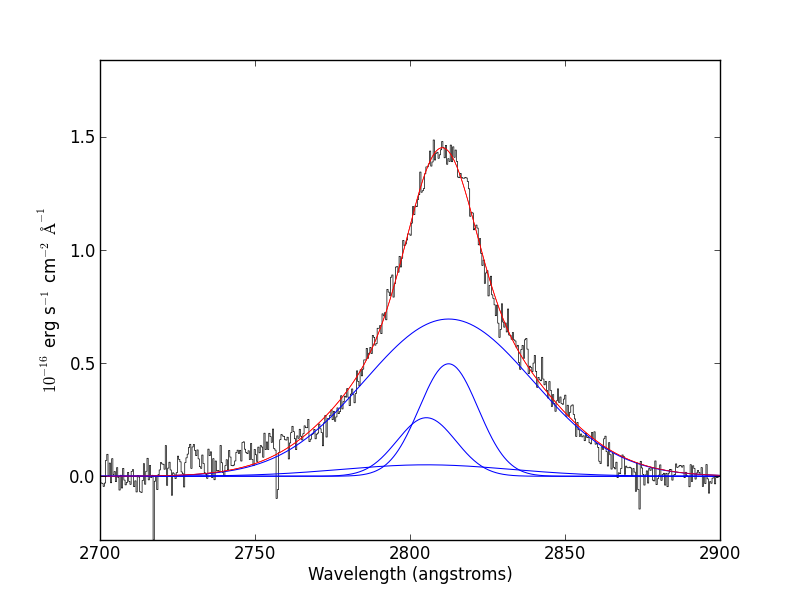
\includegraphics[width=0.46\linewidth,angle=0]{MgII_0.png}
\vspace{5mm}
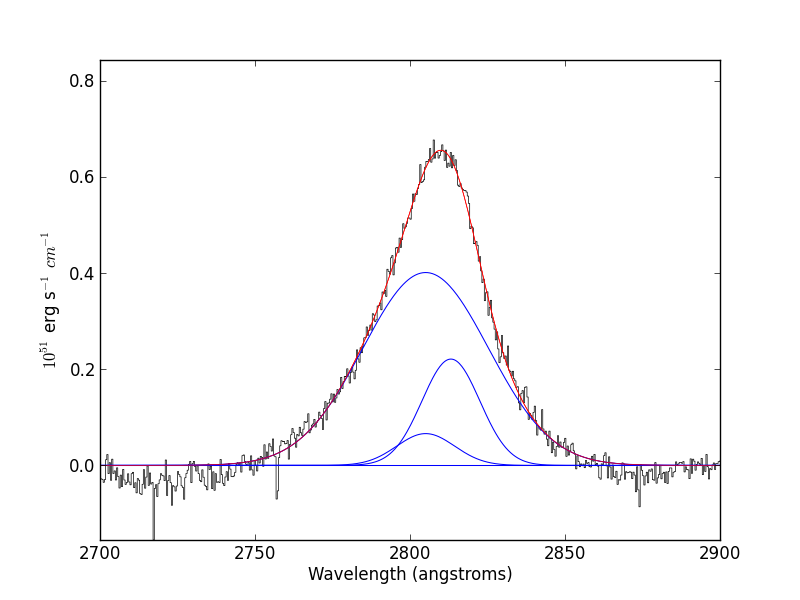
\includegraphics[width=0.49\linewidth,angle=0]{MgII_1.png}\\
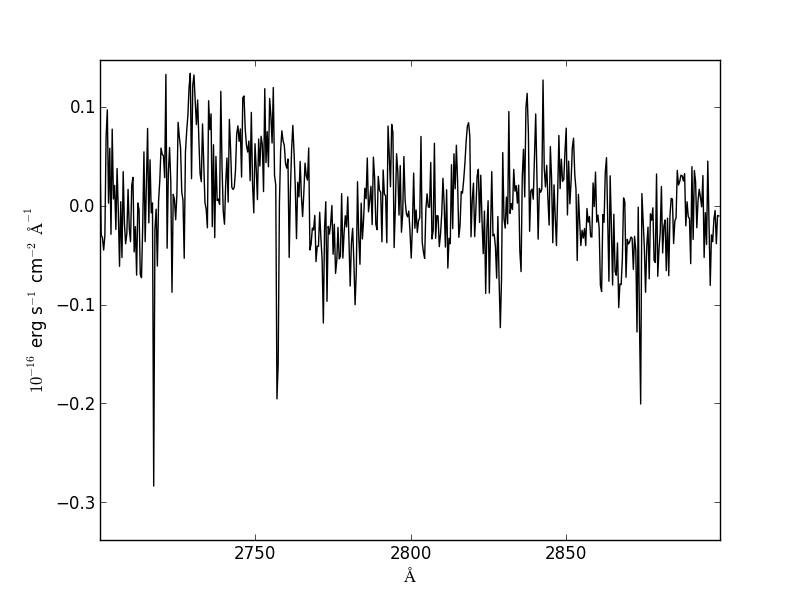
\includegraphics[width=0.46\linewidth,angle=0]{MgII_res_0.png}
\hspace{5mm}
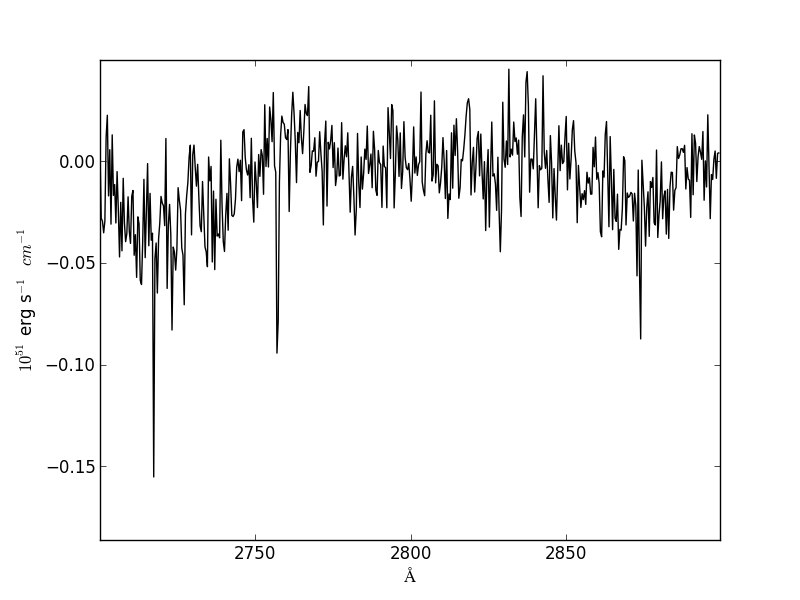
\includegraphics[width=0.49\linewidth,angle=0]{MgII_res_1.png}\\
\end{center} 
\caption{continuous fit \label{fig:landscape}}   
\end{figure*}

\newpage

\begin{figure*}
\begin{center}
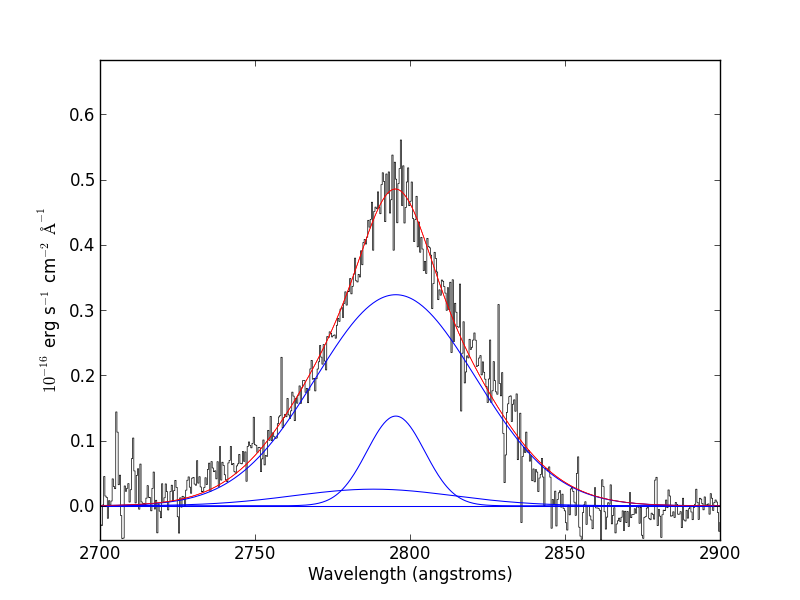
\includegraphics[width=0.46\linewidth,angle=0]{MgII_2.png}
\vspace{5mm}
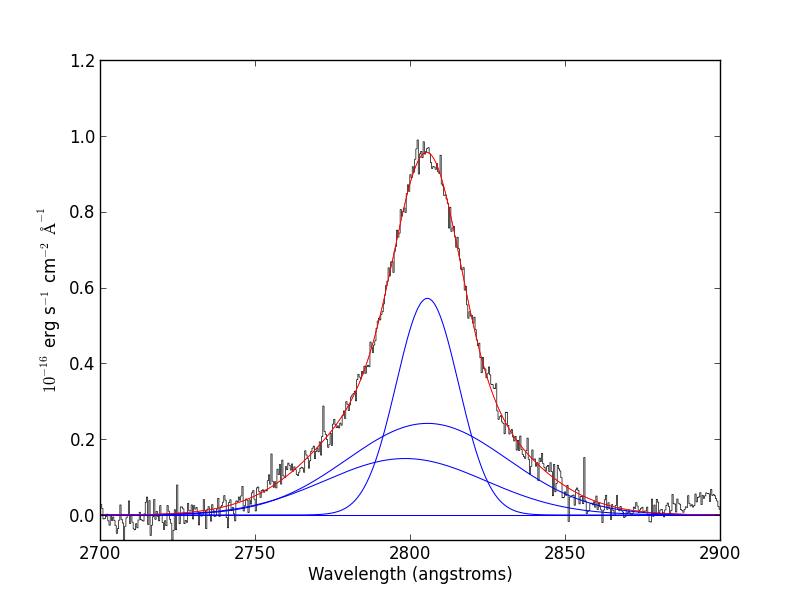
\includegraphics[width=0.49\linewidth,angle=0]{MgII_3.png}\\
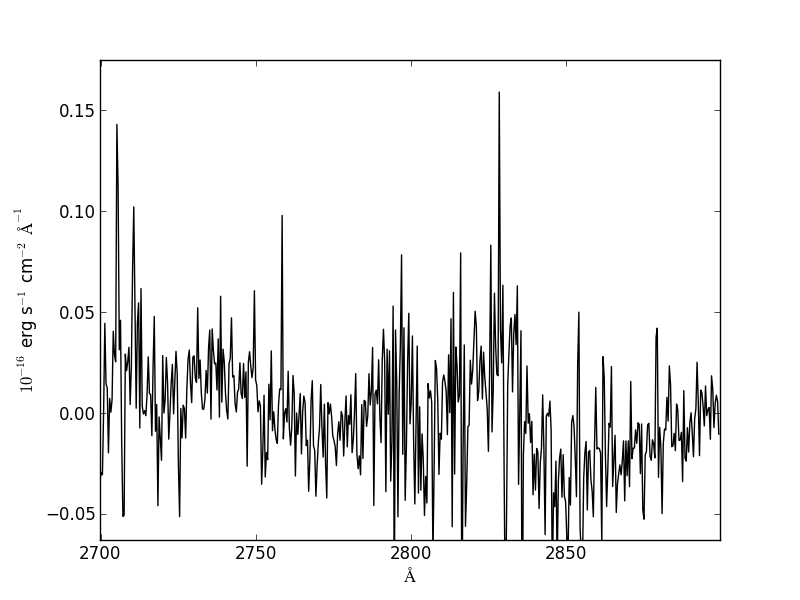
\includegraphics[width=0.46\linewidth,angle=0]{MgII_res_2.png}
\hspace{5mm}
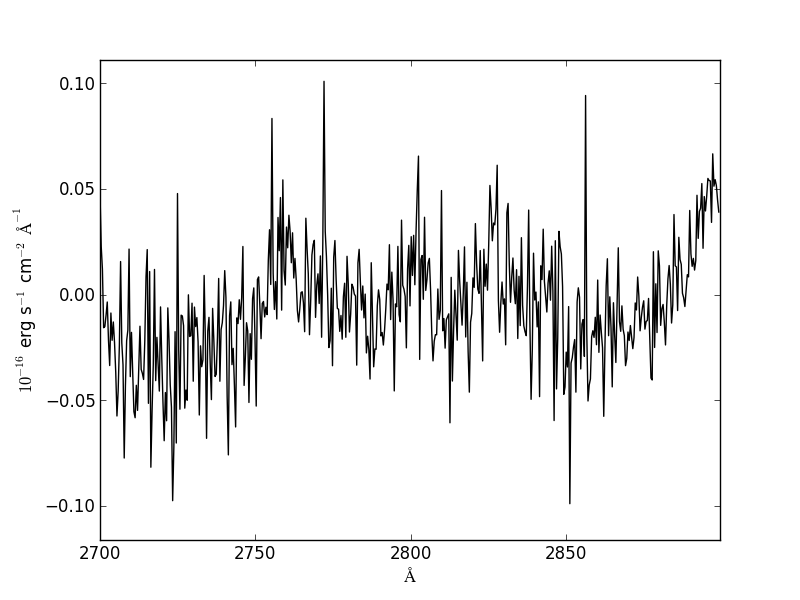
\includegraphics[width=0.49\linewidth,angle=0]{MgII_res_3.png}\\
\end{center} 
\caption{continuous fit \label{fig:landscape}}   
\end{figure*}

\newpage


\begin{figure*}
\begin{center}
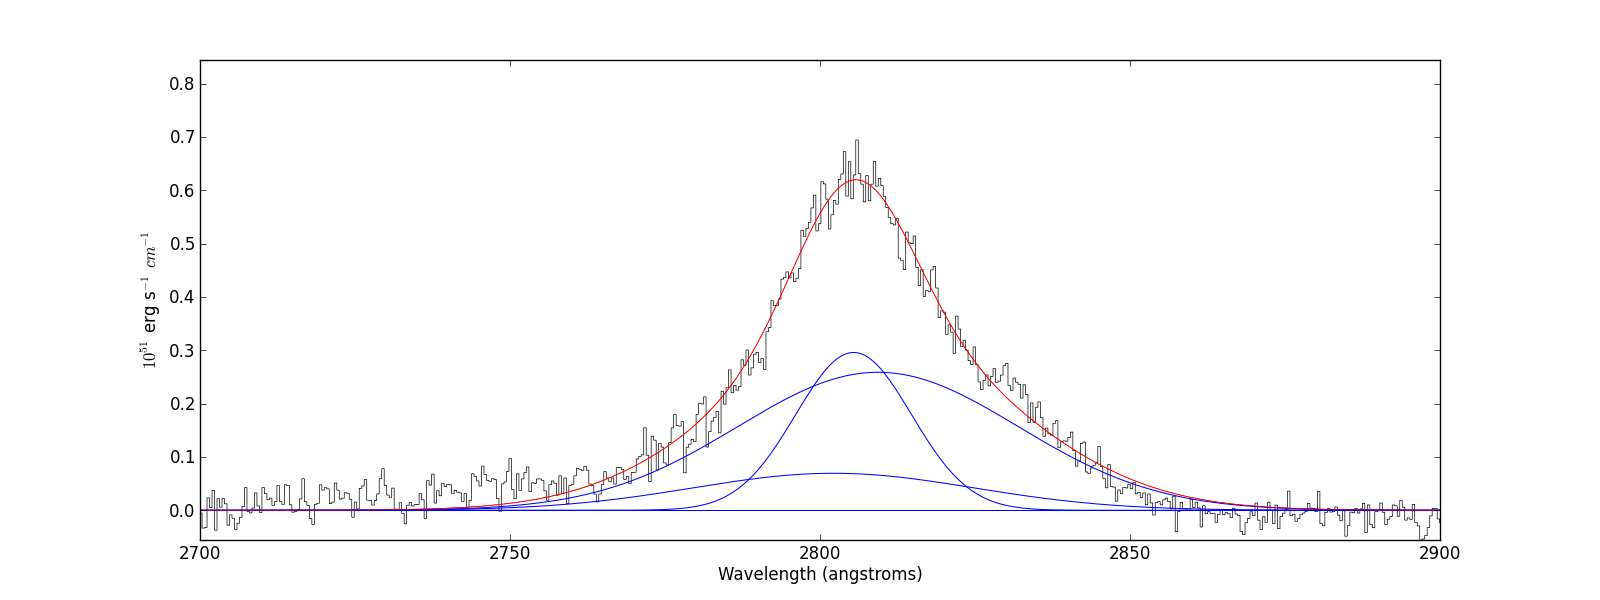
\includegraphics[width=0.46\linewidth,angle=0]{MgII_4.png}
\vspace{5mm}
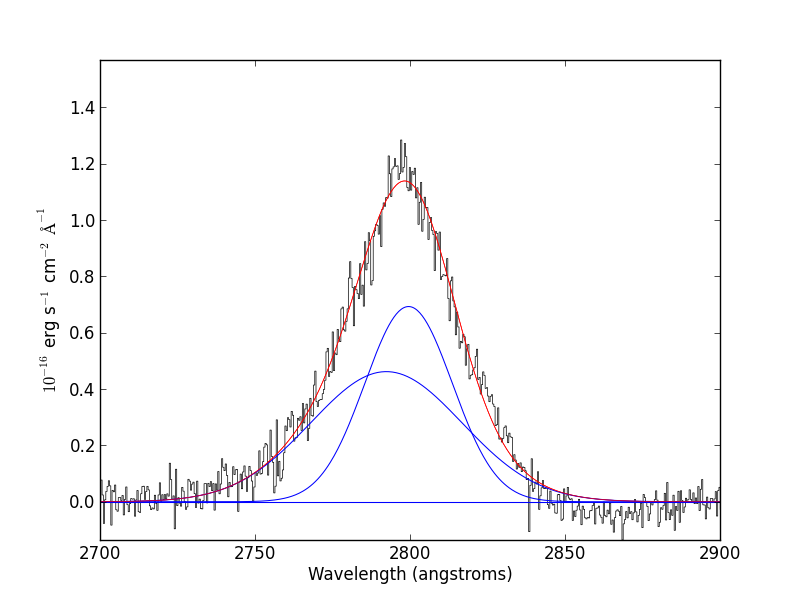
\includegraphics[width=0.49\linewidth,angle=0]{MgII_5.png}\\
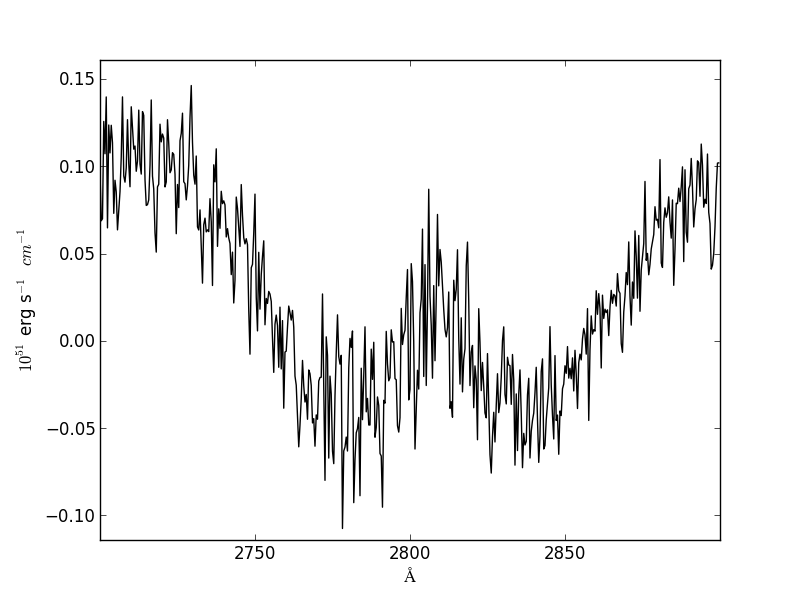
\includegraphics[width=0.46\linewidth,angle=0]{MgII_res_4.png}
\hspace{5mm}
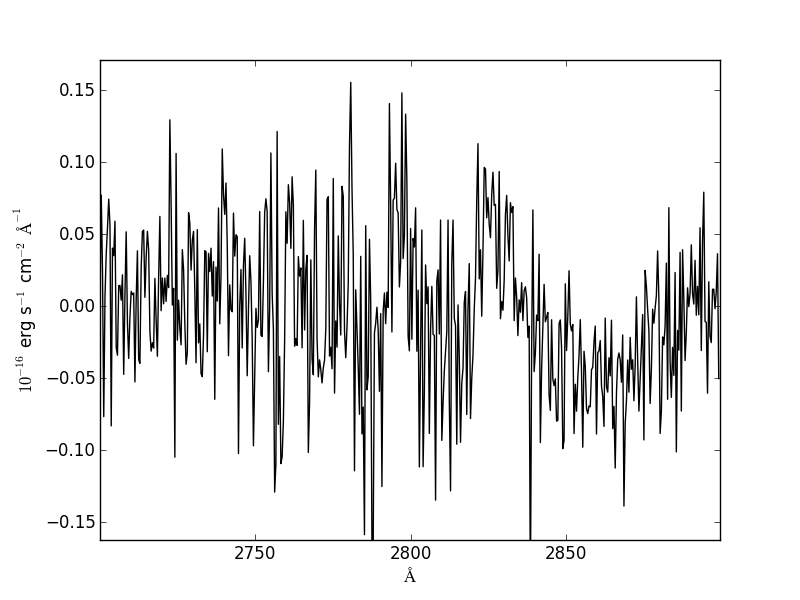
\includegraphics[width=0.49\linewidth,angle=0]{MgII_res_5.png}\\
\end{center} 
\caption{continuous fit \label{fig:landscape}}   
\end{figure*}

\newpage


\begin{figure*}
\begin{center}
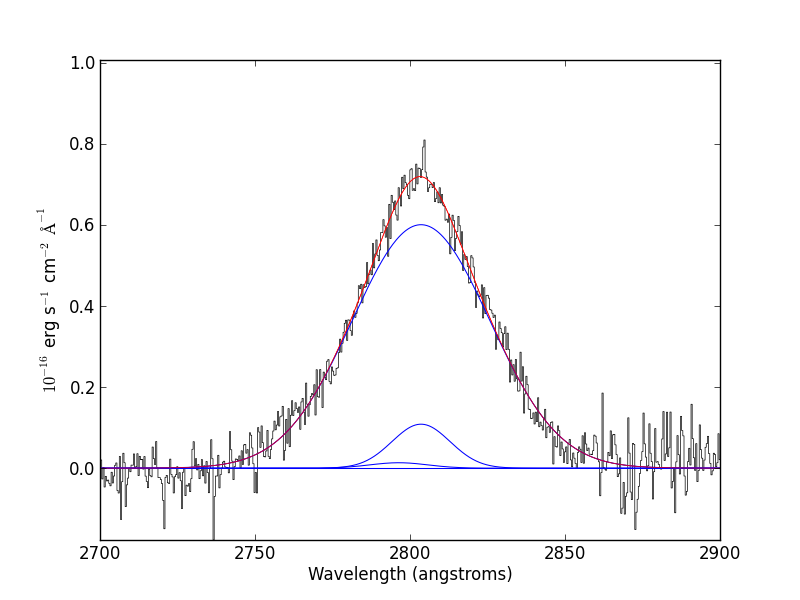
\includegraphics[width=0.46\linewidth,angle=0]{MgII_6.png}
\vspace{5mm}
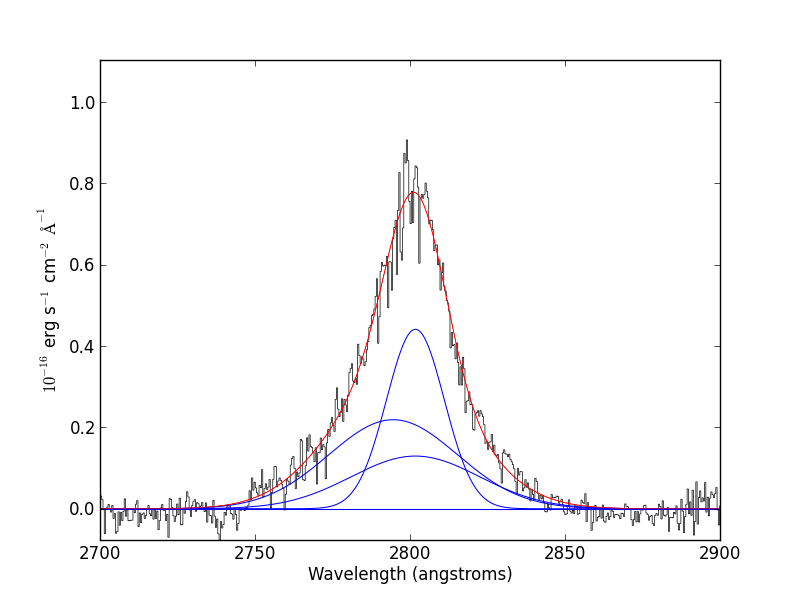
\includegraphics[width=0.49\linewidth,angle=0]{MgII_7.png}\\
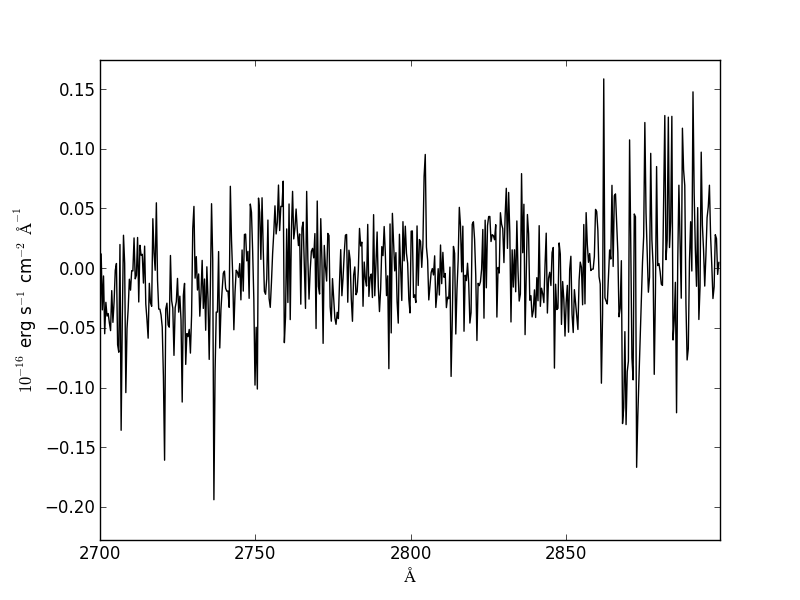
\includegraphics[width=0.46\linewidth,angle=0]{MgII_res_6.png}
\hspace{5mm}
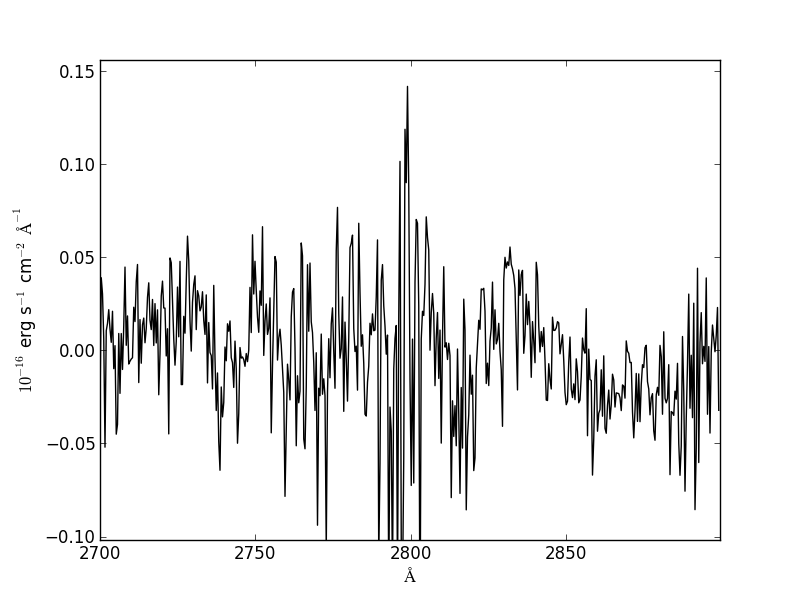
\includegraphics[width=0.49\linewidth,angle=0]{MgII_res_7.png}\\
\end{center} 
\caption{continuous fit \label{fig:landscape}}   
\end{figure*}

\newpage

\begin{figure*}
\begin{center}
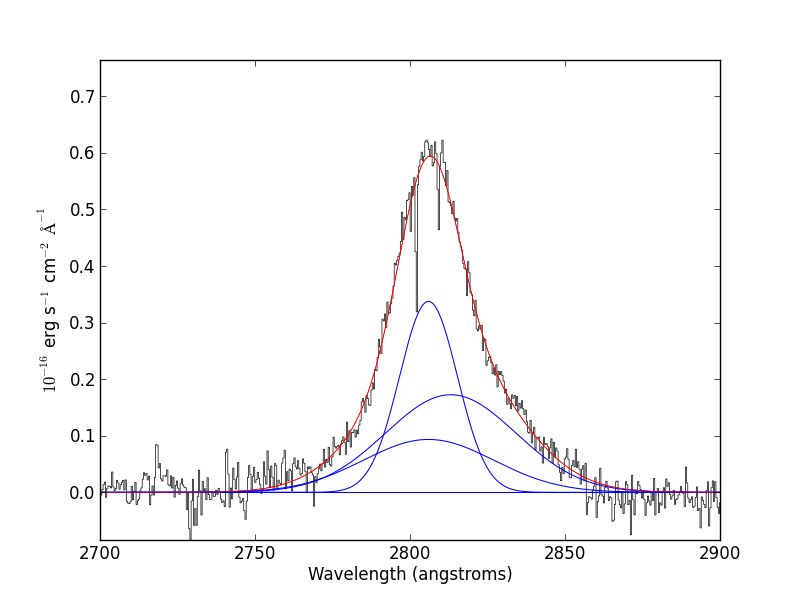
\includegraphics[width=0.46\linewidth,angle=0]{MgII_8.png}
\vspace{5mm}
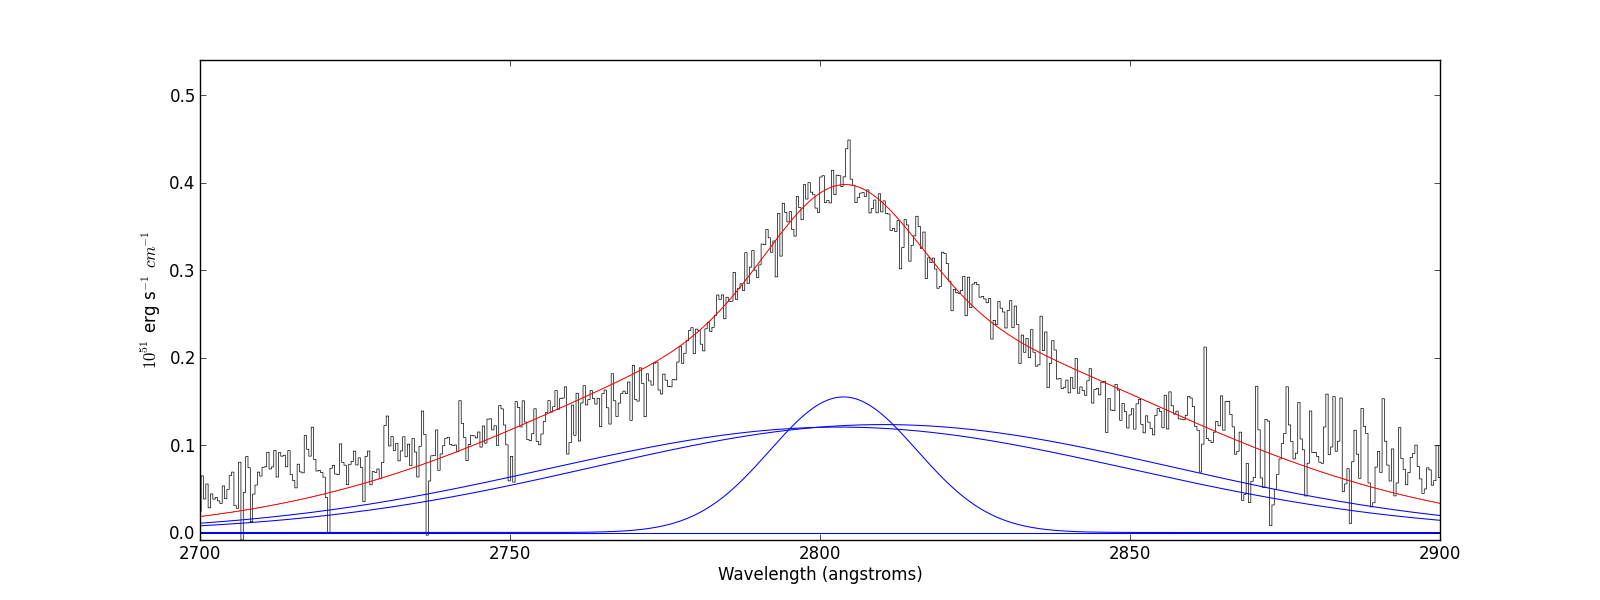
\includegraphics[width=0.49\linewidth,angle=0]{MgII_9.png}\\
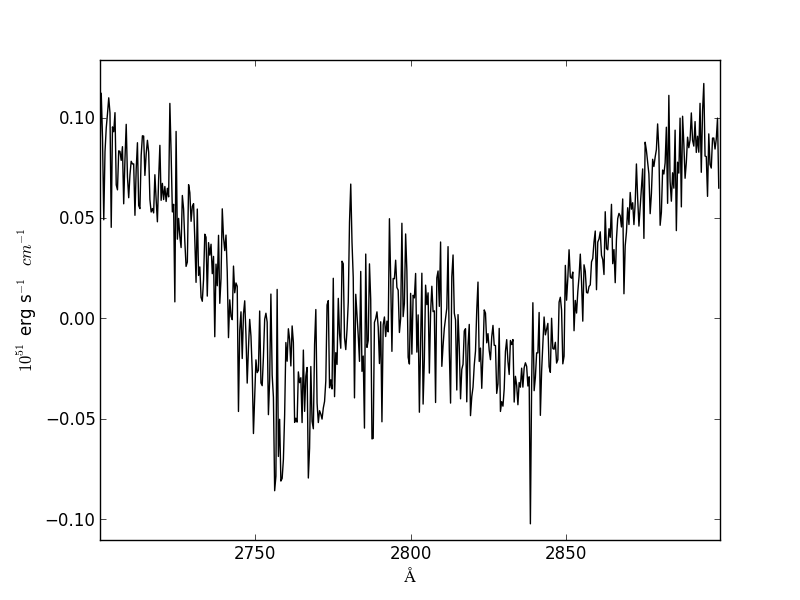
\includegraphics[width=0.46\linewidth,angle=0]{MgII_res_8.png}
\hspace{5mm}
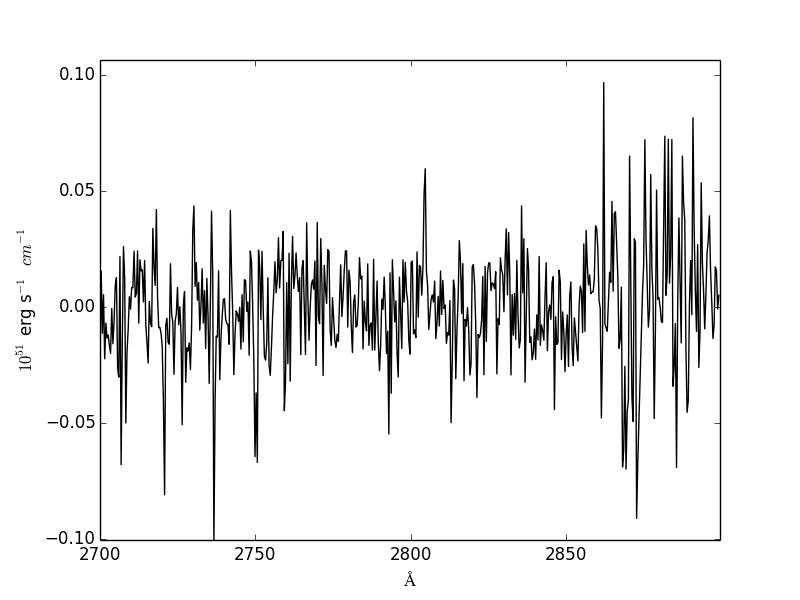
\includegraphics[width=0.49\linewidth,angle=0]{MgII_res_9.png}\\
\end{center} 
\caption{continuous fit \label{fig:landscape}}   
\end{figure*}

\newpage



\section{Hbeta}

%\subsection{Fe_fit}

\begin{figure*}
\begin{center}
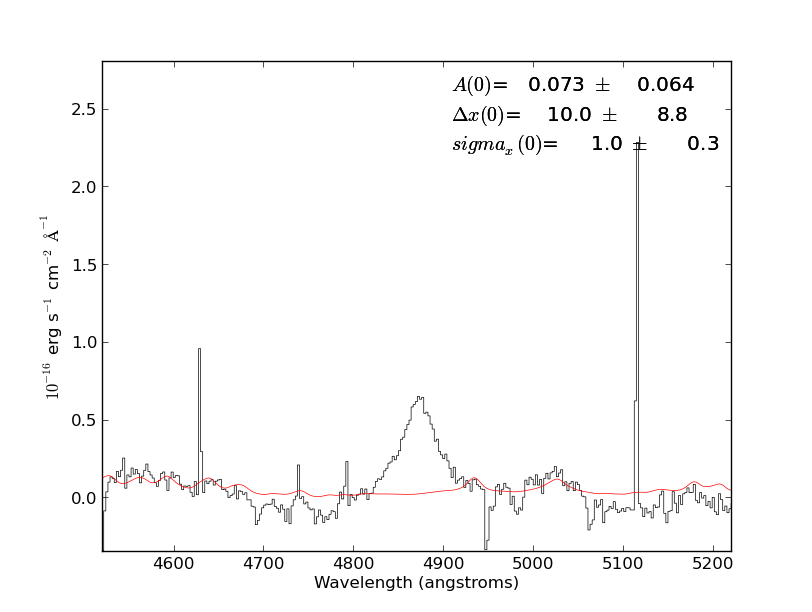
\includegraphics[width=0.46\linewidth,angle=0]{fe_fit_Hbeta_0.png}
\vspace{5mm}
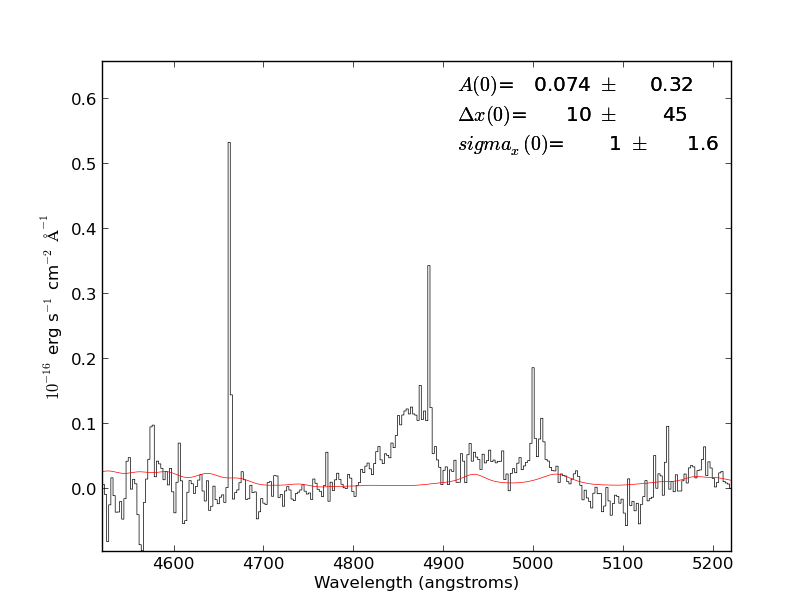
\includegraphics[width=0.49\linewidth,angle=0]{fe_fit_Hbeta_1.png}\\
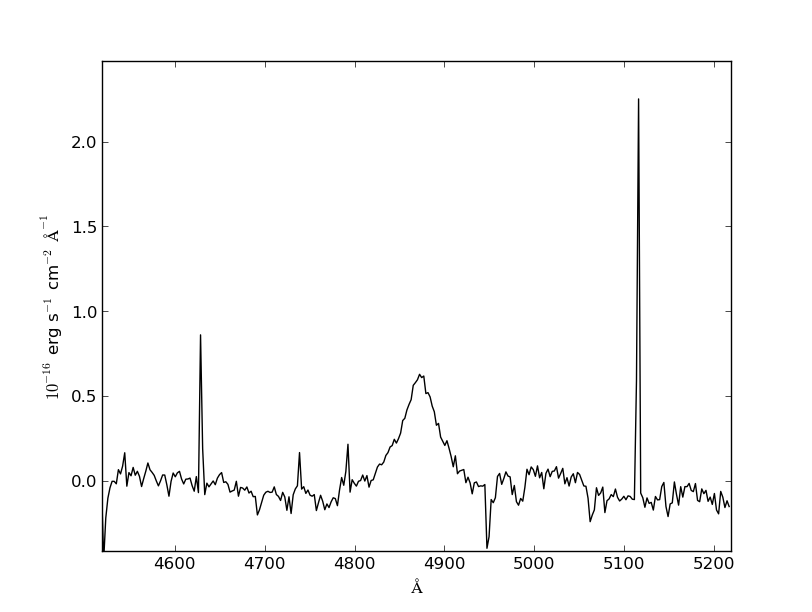
\includegraphics[width=0.46\linewidth,angle=0]{fe_fit_Hbeta_res_0.png}
\hspace{5mm}
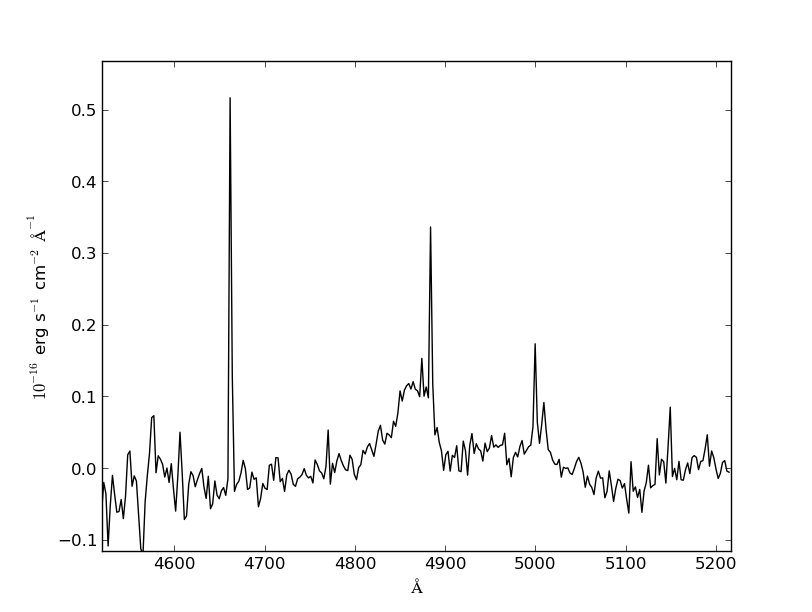
\includegraphics[width=0.49\linewidth,angle=0]{fe_fit_Hbeta_res_1.png}\\
\end{center} 
\caption{continuous fit \label{fig:landscape}}   
\end{figure*}

\newpage

\begin{figure*}
\begin{center}
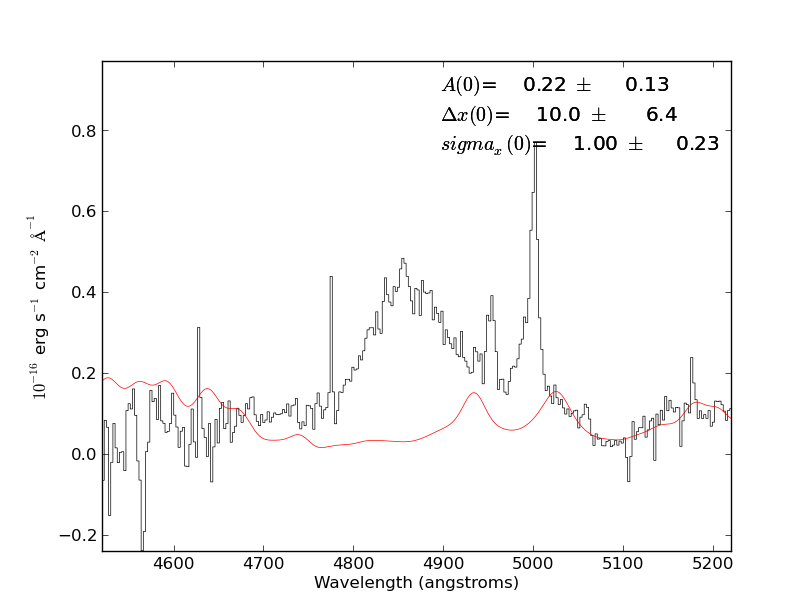
\includegraphics[width=0.46\linewidth,angle=0]{fe_fit_Hbeta_2.png}
\vspace{5mm}
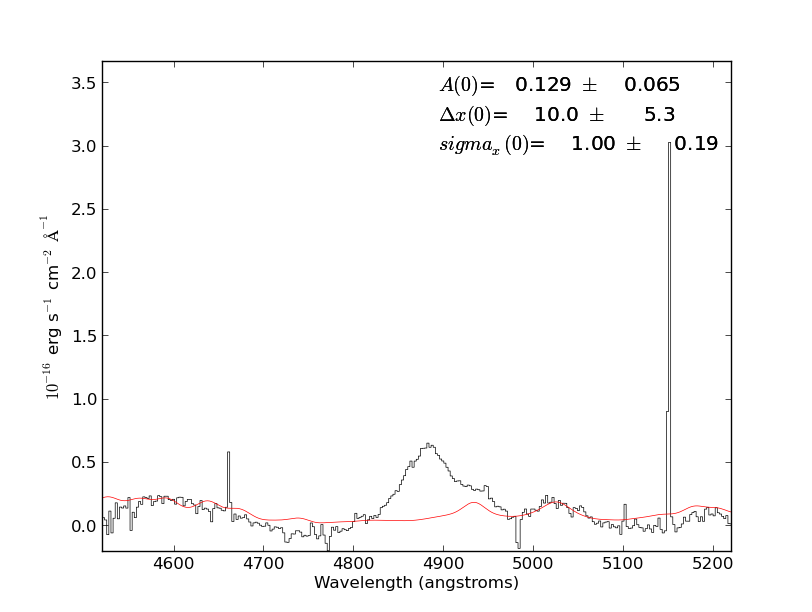
\includegraphics[width=0.49\linewidth,angle=0]{fe_fit_Hbeta_3.png}\\
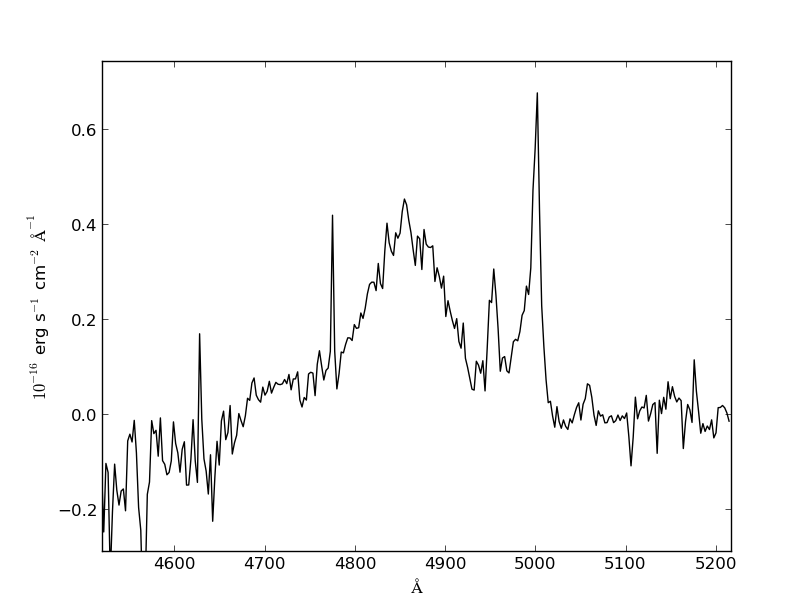
\includegraphics[width=0.46\linewidth,angle=0]{fe_fit_Hbeta_res_2.png}
\hspace{5mm}
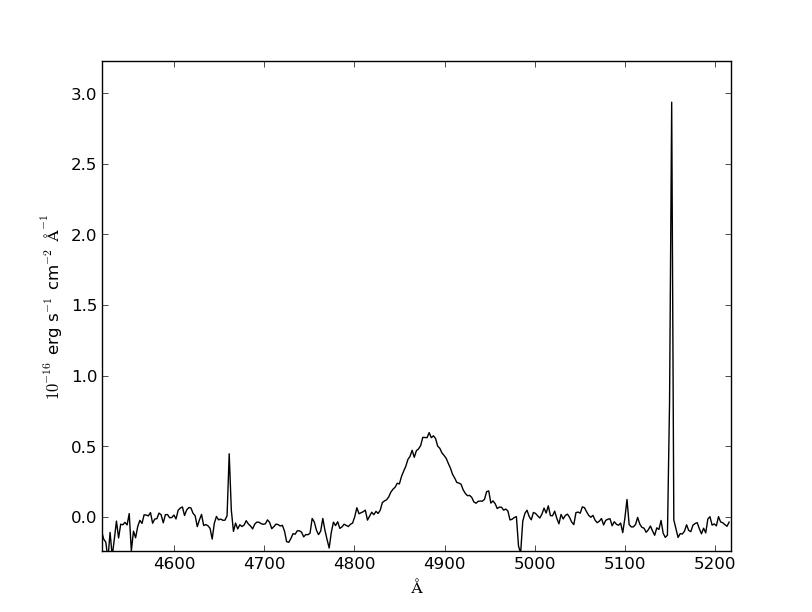
\includegraphics[width=0.49\linewidth,angle=0]{fe_fit_Hbeta_res_3.png}\\
\end{center} 
\caption{continuous fit \label{fig:landscape}}   
\end{figure*}

\newpage


\begin{figure*}
\begin{center}
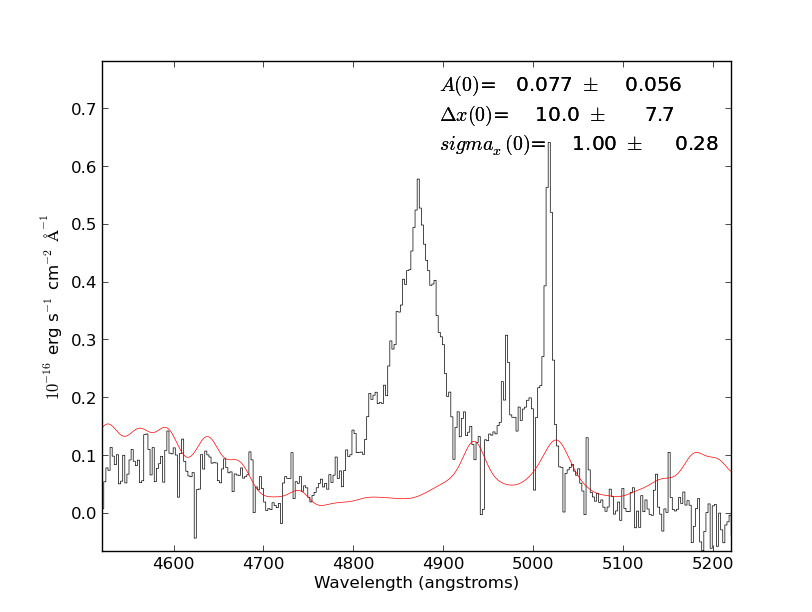
\includegraphics[width=0.46\linewidth,angle=0]{fe_fit_Hbeta_4.png}
\vspace{5mm}
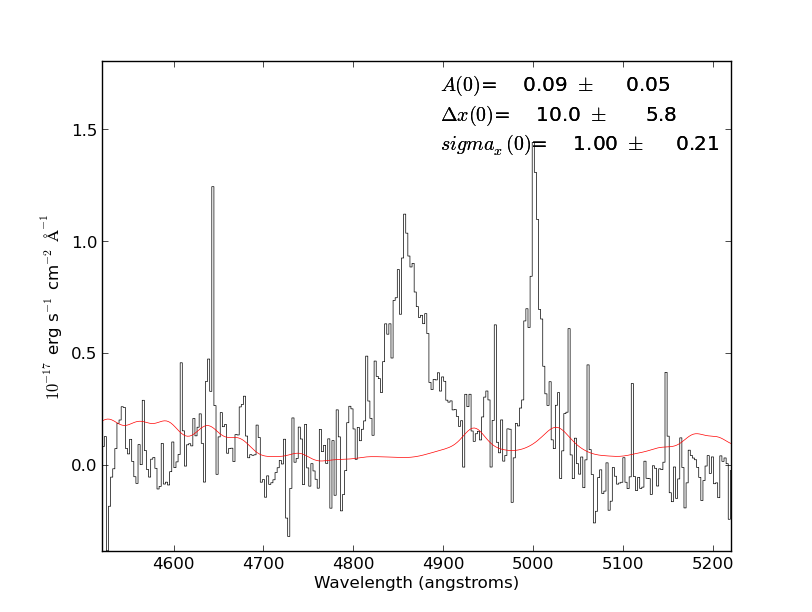
\includegraphics[width=0.49\linewidth,angle=0]{fe_fit_Hbeta_5.png}\\
\includegraphics[width=0.46\linewidth,angle=0]{fe_fit_Hbeta_res_4.png}
\hspace{5mm}
\includegraphics[width=0.49\linewidth,angle=0]{fe_fit_Hbeta_res_5.png}\\
\end{center} 
\caption{continuous fit \label{fig:landscape}}   
\end{figure*}

\newpage


\begin{figure*}
\begin{center}
\includegraphics[width=0.46\linewidth,angle=0]{fe_fit_Hbeta_6.png}
\vspace{5mm}
\includegraphics[width=0.49\linewidth,angle=0]{fe_fit_Hbeta_7.png}\\
\includegraphics[width=0.46\linewidth,angle=0]{fe_fit_Hbeta_res_6.png}
\hspace{5mm}
\includegraphics[width=0.49\linewidth,angle=0]{fe_fit_Hbeta_res_7.png}\\
\end{center} 
\caption{continuous fit \label{fig:landscape}}   
\end{figure*}

\newpage

\begin{figure*}
\begin{center}
\includegraphics[width=0.46\linewidth,angle=0]{fe_fit_Hbeta_8.png}
\vspace{5mm}
\includegraphics[width=0.49\linewidth,angle=0]{fe_fit_Hbeta_9.png}\\
\includegraphics[width=0.46\linewidth,angle=0]{fe_fit_Hbeta_res_8.png}
\hspace{5mm}
\includegraphics[width=0.49\linewidth,angle=0]{fe_fit_Hbeta_res_9.png}\\
\end{center} 
\caption{continuous fit \label{fig:landscape}}   
\end{figure*}

\newpage


\section{Hbeta fit}

\begin{figure*}
\begin{center}
\includegraphics[width=0.46\linewidth,angle=0]{Hbeta_0.png}
\vspace{5mm}
\includegraphics[width=0.49\linewidth,angle=0]{Hbeta_1.png}\\
\includegraphics[width=0.46\linewidth,angle=0]{Hbeta_res_0.png}
\hspace{5mm}
\includegraphics[width=0.49\linewidth,angle=0]{Hbeta_res_1.png}\\
\end{center} 
\caption{continuous fit \label{fig:landscape}}   
\end{figure*}

\newpage

\begin{figure*}
\begin{center}
\includegraphics[width=0.46\linewidth,angle=0]{Hbeta_2.png}
\vspace{5mm}
\includegraphics[width=0.49\linewidth,angle=0]{Hbeta_3.png}\\
\includegraphics[width=0.46\linewidth,angle=0]{Hbeta_res_2.png}
\hspace{5mm}
\includegraphics[width=0.49\linewidth,angle=0]{Hbeta_res_3.png}\\
\end{center} 
\caption{continuous fit \label{fig:landscape}}   
\end{figure*}

\newpage


\begin{figure*}
\begin{center}
\includegraphics[width=0.46\linewidth,angle=0]{Hbeta_4.png}
\vspace{5mm}
\includegraphics[width=0.49\linewidth,angle=0]{Hbeta_5.png}\\
\includegraphics[width=0.46\linewidth,angle=0]{Hbeta_res_4.png}
\hspace{5mm}
\includegraphics[width=0.49\linewidth,angle=0]{Hbeta_res_5.png}\\
\end{center} 
\caption{continuous fit \label{fig:landscape}}   
\end{figure*}

\newpage


\begin{figure*}
\begin{center}
\includegraphics[width=0.46\linewidth,angle=0]{Hbeta_6.png}
\vspace{5mm}
\includegraphics[width=0.49\linewidth,angle=0]{Hbeta_7.png}\\
\includegraphics[width=0.46\linewidth,angle=0]{Hbeta_res_6.png}
\hspace{5mm}
\includegraphics[width=0.49\linewidth,angle=0]{Hbeta_res_7.png}\\
\end{center} 
\caption{continuous fit \label{fig:landscape}}   
\end{figure*}

\newpage

\begin{figure*}
\begin{center}
\includegraphics[width=0.46\linewidth,angle=0]{Hbeta_8.png}
\vspace{5mm}
\includegraphics[width=0.49\linewidth,angle=0]{Hbeta_9.png}\\
\includegraphics[width=0.46\linewidth,angle=0]{Hbeta_res_8.png}
\hspace{5mm}
\includegraphics[width=0.49\linewidth,angle=0]{Hbeta_res_9.png}\\
\end{center} 
\caption{continuous fit \label{fig:landscape}}   
\end{figure*}

\newpage


\end{document}
